% Copyright (c) 2014,2016,2018 Casper Ti. Vector
% Public domain.

\chapter{LHC and \lhcb }
\label{chap:lhcb}
%\pkuthssffaq % 中文测试文字。

The data collected from proton-proton collisions is used in this disseration,
which is generated by the Large Hadron Collider(LHC) and collected in LHCb experiment,
so a brief overview of LHC and \lhcb during Run 1 and Run 2 will be given in this chapter.
Currently, 
the \lhcb sub-detectors are being upgraded for higher luminosity situation in the following Run 3 era, 
the \upgradeone scenario for each subdetector will also be mentioned.  
As this disseration includes some \ecal simulation results for \lhcb \upgradetwo,
more detailed description related to \lhcb calorimeter system will be reviewed in this chapter.

\section{The large hadron collider}

LHC, 
an international project at the European Organization for Nuclear Research (CERN) laboratory in Geneva, Switzerland, 
is the most powerful particle accelerator ever constructed. 
It produces the highest energy particle beams ever created, 
making it the premier facility in the world for research in elementary particle physics. 
The LHC consists of a superconducting particle accelerator, 
approximately 27 kelometers in circumference, 
providing two counter-rotating proton beams with a design energy of 7 TeV per beam. 
It can also provide colliding beams of heavy ions, such as lead. 
During 2011 and 2012 (Run1) the LHC operated at 4 TeV per beam because of a limitation in the electrical connections
between the superconducting magnets. 
After the connections were upgraded during a nearly two-year shutdown, 
Run2 began in mid-2015 and lasted to the end of 2018 at 6.5 TeV per beam,
exploring a new energy region not accessible during Run1. 

\begin{figure}[!hbtp]
\centering
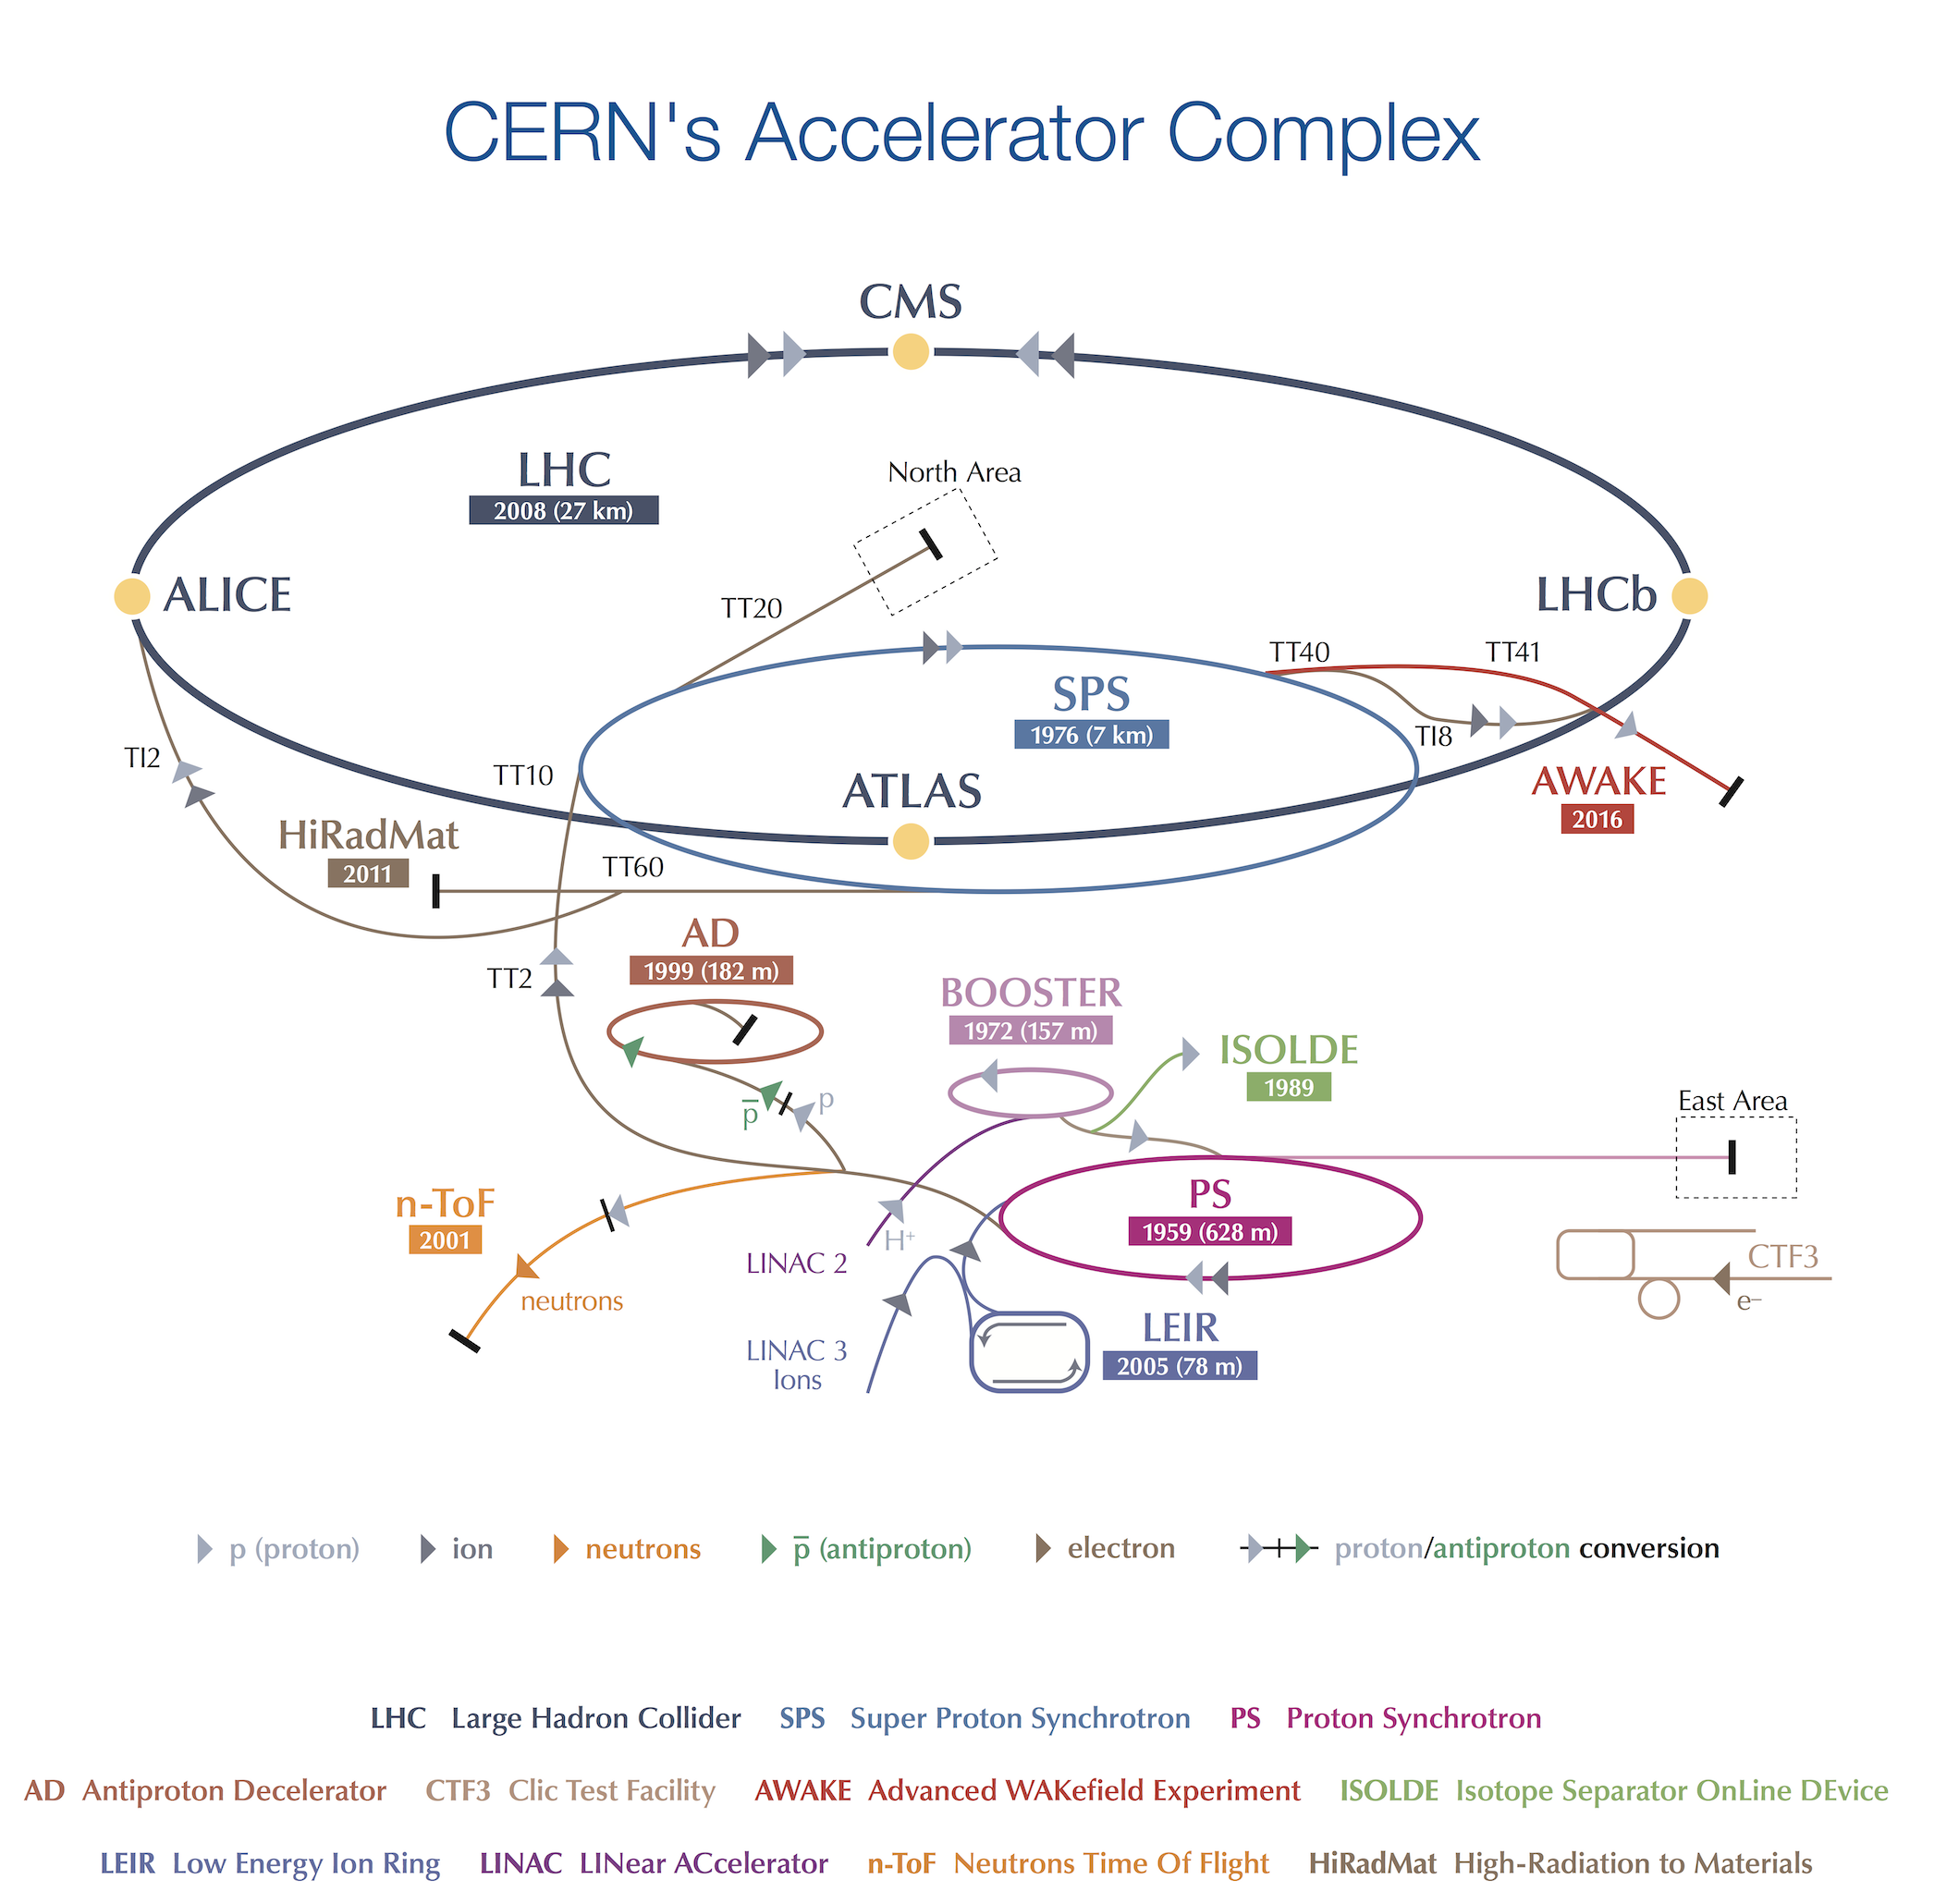
\includegraphics[width=1\textwidth]{Figures/02_Detector/LHC}%
\caption{The CERN accelerator complex.
The LHC is the last ring (dark grey line) in a complex chain of particle accelerators. 
The smaller machines are used in a chain to help boost the particles to their final energies and provide beams to a whole set of smaller experiments, 
which also aim to uncover the mysteries of the Universe\supercite{Haffner:1621894}.}
\label{fig:LHC}
\end{figure}


Actually, 
the LHC is the last element of accelerator complex at CERN,
which is a succession of machines that accelerate particles to increasingly higher energies, as shown in Figure.~\ref{fig:LHC}.
Each machine in the complex boosts the energy of a beam of particles, before injecting the beam into the next machine in the sequence. 
Most of the other accelerators in the chain have their own experimental halls where beams are used for experiments at lower energies.

The proton source comes from a simple bottle of hydrogen gas. 
Then, 
electric field is used to strip the electrons in hydrogen atoms to create protons. 
Linac 2, 
the first accelerator in the complex, 
accelerates the protons to the energy of 50 MeV. 
%Afterwards, 
Subsequently,
the beam is then injected into the Proton Synchrotron Booster (PSB), 
which accelerates the protons to 1.4 GeV, 
afterwards, the Proton Synchrotron (PS) pushes the beam to 25 GeV. 
Then, 
protons are sent to the Super Proton Synchrotron (SPS) which accelerates them to 450 GeV.
Finally, 
the protons are transferred to the two beam pipes of the LHC. 
Two beams in LHC circulate clockwise or anticlockwise respectively.
It takes around 4 minutes to fill each LHC ring, 
and 20 minutes for the protons to reach their maximum energy of 6.5 TeV. 
Beams run for several hours inside the LHC beam pipes under normal operating conditions. 
The two beams collide inside four detectors, 
ALICE, ATLAS, CMS and \lhcb, 
in which the total energy at the collision point is equal to 13 TeV.
The accelerator complex is the Antiproton Decelerator and the Online Isotope Mass Separator (ISOLDE) facility, 
and the Compact Linear Collider test area, 
as well as the neutron time-of-flight facility (nTOF). 
It also provides beams to Gran Sasso (CNGS) project for neutino experiment.
Besides,
protons are not the only particles accelerated in the LHC,
In addition to the protons,
lead ions can be accelerated in LHC,
which start from a source of vaporised lead and enter Linac 3 before being collected, 
they then follow the same route to maximum energy as the protons.

\begin{figure}[!hbtp]
\centering
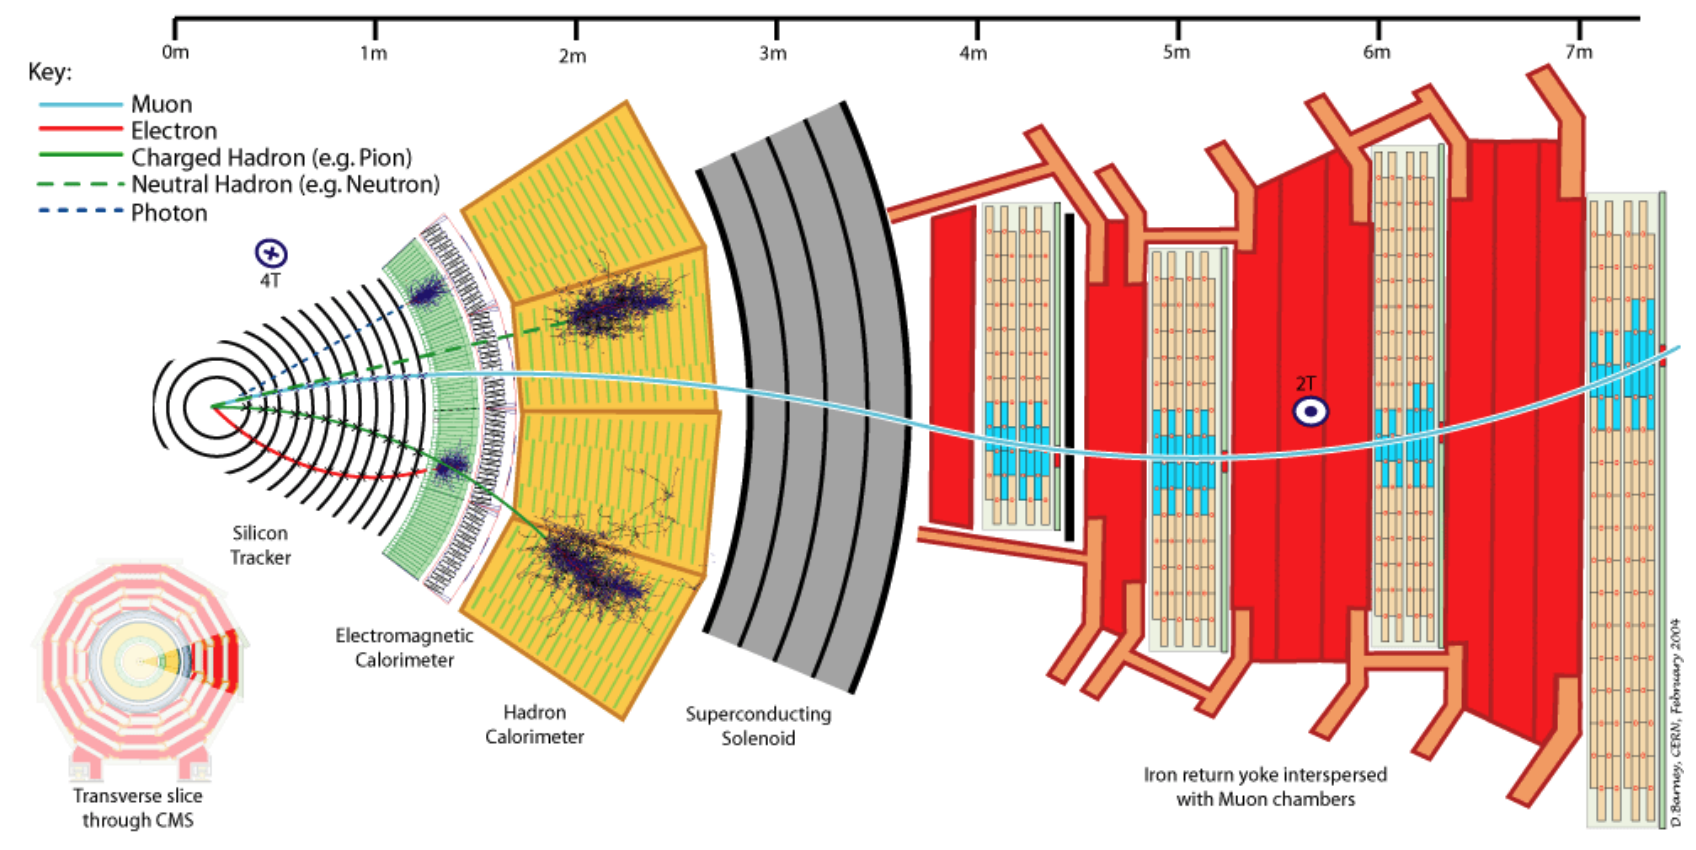
\includegraphics[width=0.7\textwidth]{Figures/02_Detector/CMS}%
\caption{Transverse slice through the CMS detector,
the particle type can be inferred by combining the detector response in the different subdetectors.\supercite{Nielsen_2011}.}
\label{fig:CMS}
\end{figure}

Four main experiments are placed at the LHC. 
Two of them are general purpose experiments, 
studying many aspects of particle productions and decaies. 
These are ATLAS (A Toroidal LHC Apparatus) and CMS (Compact Muon Solenoid) experiments, 
each of them involves more than 3000 scientists and engineers,
in order to search particles beyond standard model directly.
The other experiments, 
each involving around 1000 scientists and engineers, 
and the physical destinations are more specialised: ALICE, (A Large Ion-Collider Experiment) is concerned with heavy-ion collisions, 
and \lhcb (LHC b-hadron experiment) focuses more on the decays of hadrons containing the bottom quark.

These detectors have been constructed as a series of subdetectors, 
and all follow roughly the same scheme,
as shown in Figure.~\ref{fig:CMS},
where the CMS is taken as an example. 
Starting from the inner layers, 
which are positioned closest to the interaction region, 
each detector consists of: 
subdetectors to measure charged-particle trajectories; 
subdetectors to stop photons, 
electrons and hadrons, 
and measure their energies; 
subdetectors to record muons, 
the only charged particles that reach the detector’s outermost layers. 
The ALICE, ATLAS and CMS detectors are approximately cylindrical in shape, 
so as to be sensitive to particles emerging in all directions from an interaction. 
The majority of the particles of interest in \lhcb are emitted at small angles, 
and so the experiment’s detector covers only a narrow cone around the direction of the incoming protons.
In next section, 
the detailed structure of \lhcb will be reviewed.


\section{The \lhcb detector}
LHCb is a single-arm spectrometer with a forward angular coverage from approximately 10 mrad to 300 (250) \mrad,
corresponding to a pseudorapidity range of $1.8 <\eta < 4.9$. 
The layout of the LHCb spectrometer is shown in Figure.~\ref{fig:LHCb}. 
The right-handed coordinate system adopted has the z axis along the beam, and the y axis along the vertical.
This particular geometry of the detector was chosen as the production of \bquark and \bquarkbar quarks at LHC energies 
is such that their directions will tend to be along the beam line.
The polar angles of the \bquark and \bquarkbar hadrons produced for $\sqs=8\tev$ collisions are shown in Figure.~\ref{fig:BBar}, 
as predicted from \pythia8 simulations\supercite{SJOSTRAND2008852},
and similar results apply for pp collisions with the centre-of-mass energy ranging from 7\tev to 14 \tev.
%The choice of the detector geometry is justified by the fact 
%that at high energies both the \bquark-hadrons are predominantly produced in the same forward or backward cone.

\begin{figure}[!hbtp]
\centering
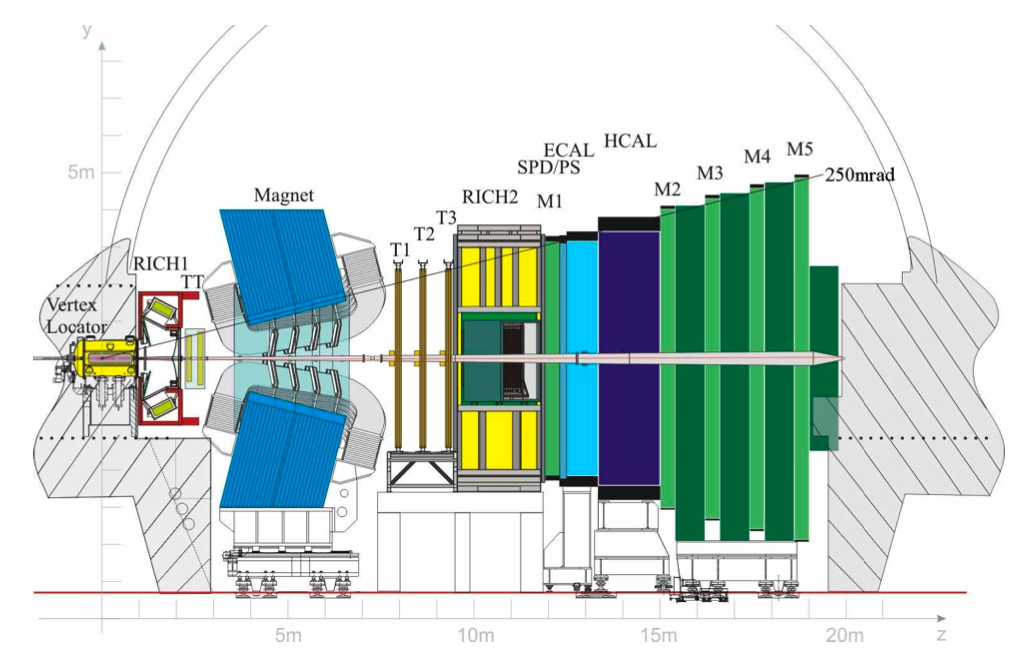
\includegraphics[width=0.95\textwidth]{Figures/02_Detector/LHCb}%
\caption{View of the \lhcb detector\supercite{LHCb-DP-2008-001}.}
\label{fig:LHCb}
\end{figure}

\begin{figure}[!hbtp]
\centering
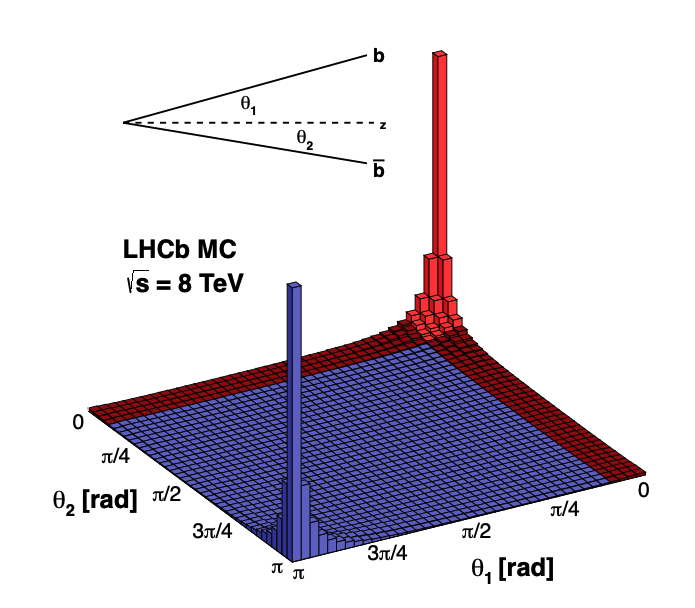
\includegraphics[width=0.65\textwidth]{Figures/02_Detector/BBbar}%
\caption{Display of $\bquark\bquarkbar$ production angles as simulated with \pythia8.
The \lhcb acceptance is shown in red.}
\label{fig:BBar}
\end{figure}

The detector during Run1 and Run2 was designed to operate at a luminosity of $\lum=2\times10^{32}\cm^{-2}s^{-1}$, 
considering the LHC’s design maximum luminosity of $10^{34}\cm^{-2}s^{-1}$, 
a lower luminosity is applied to make for less “busy” events. 
Higher luminosities mean much larger number of interactions per bunch crossing, 
leading to more points where proton-proton collisions take place. 
A proton-proton collision point is also named as a primary vertex (PV), 
and the identification of primary vertices is essential in many analyses in order to accurately reconstruct the paths of decaying particles. 
A high number of primary vertices in an event makes it much more difficult to identify the primary vertex from which a particle originated. 
The higher track multiplicity events, 
which would result from more collisions, 
would also make event reconstruction more difficult. 
Moreover, operating at lower luminosities also limits the radiation damage and detector occupancy. 
A method referred to as “luminosity leveling” is used to achieve the lower luminosity. 
This is done by shifting the beams relative to each other, 
as the number of proton bunches goes down, 
the beams can be made to overlap more in small increments so that the luminosity is also kept constant.

After \upgradeone, 
the liminosity duiring LHC Run3 will be increased to $2\times10^{33}\cm^{-2}s^{-1}$,
which is around 5 times larger than the value in Run2\supercite{LHCb-TDR-012}.
After \upgradetwo,
the luminosity can reach to $1.5\times10^{34}\cm^{-2}s^{-1}$,
total around $300\invfb$ of data will be recorded, 
which offer us an opportunity to take full advantage of the flavour-physics opportunities at the HL-LHC\supercite{LHCb-PII-EoI,LHCb-PII-Physics}.
More comments to \upgradetwo and corresponding the chellange to detector upgrade will be discussed in Chapter\ref{chap:ecal},
especially about \ecal.


\subsection{Tracking}

The tracking system are used to reconstruct charged particles,
and the particles go through tracking subdetectors in proper sequence,
which cantains several parts at \lhcb, 
the Vertex Locater (VELO), 
Diple Magnets and four tracking stations,
as shown in Figure.~\ref{fig:Tracking}.
When comes to the four stations,
one is set in the front of magnet field, 
refered as Tracker Turicensis (TT) and constructed using silicon microstrip sensors,
and other three are located behind the magnet,
known as T1, T2 and T3.
These three stations are divided into inner and outer parts,
the inner section is built by slicon microstrip, 
called as Inner Tracker (IT),
while the outer part is a drift-time dector,
referred to as Outer Tracker (OT).
The following is some details about these sub-detectors.

\begin{figure}[!hbtp]
\centering
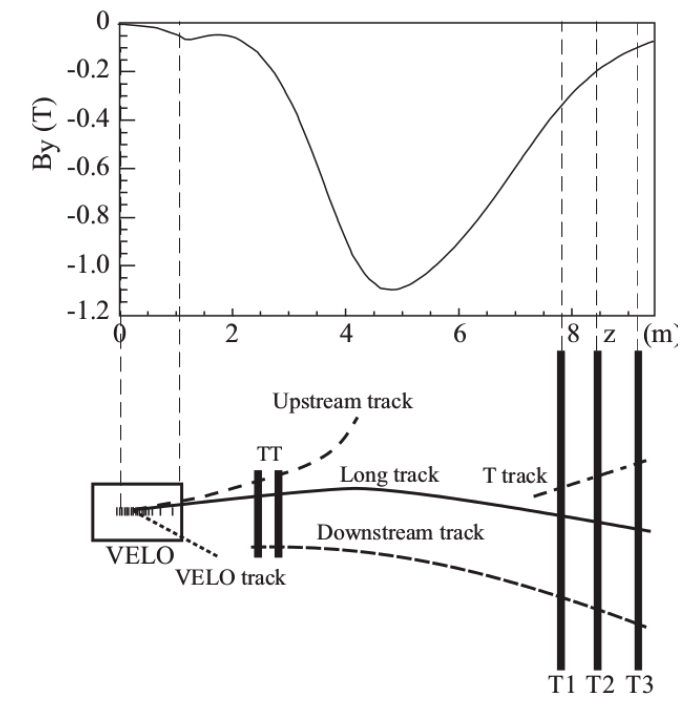
\includegraphics[width=0.65\textwidth]{Figures/02_Detector/Tracking}%
\caption{ Schematic of the tracking compoents with different types of tracking definitions in the tracking reconstruction\supercite{LHCb-DP-2014-002}}
\label{fig:Tracking}
\end{figure}


\subsubsection{Vertex Locater}

The VELO is used to reconstruct the pp collision point,
reconstruct the decay vertices of \bquark and \cquark hadrons and play an important role in second level trigger
\footnote{Details about the trigger at \lhcb will be discussed in Section~\ref{sec:trigger}.}.
For precise vertexing measuremnt,
the VELO should be put as close as possible to the decay vertices,
and make the material between the first measured point and the vertex as less as possible.

The current VELO is constructed by a series of silicon modules, 
each providing a measure of the $r$ and $\phi$ coordinates and perpendicular to the beam direction,
as shown in Figure.~\ref{fig:VELO}.
The VELO includes 25 stations, 
and all of them silicon are placed in vaccum.
Each station contants 2 modules,
positioned on left and right,
as shown in the bottom of Figure.~\ref{fig:VELO}.
Every module has 2 silicon sensors,
one is called $\phi$-measuring sensor,
provides information on the azimuthal coordinate around the beam,
the other sensor,
called the $r$-measuring sensor, 
provides information on the radial distance from the beam axis.
The total number of strips for both sensor types is about 180000 channels.

\begin{figure}[!hbtp]
\centering
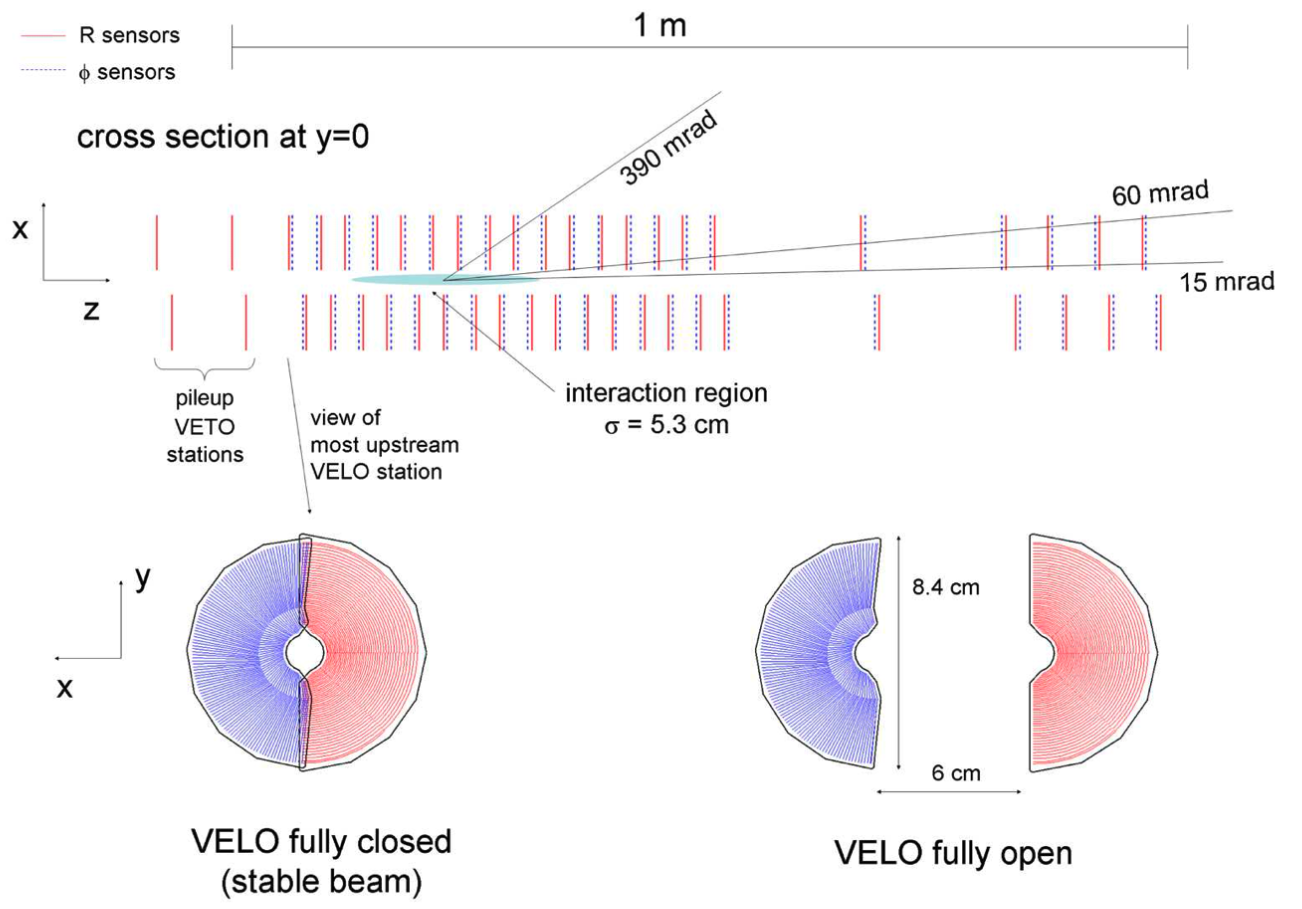
\includegraphics[width=0.85\textwidth]{Figures/02_Detector/VELO}%
\caption{ Overview of the VELO as seen in the (x, z) plane, at y=0, at top. 
	The front face of the modules in the (x,y) plane, for both closed (left) and oprn (right) positions, at bottom\supercite{LHCb-DP-2008-001}.}
\label{fig:VELO}
\end{figure}

Many auxiliary system is designed to keep \velo running normally.
As \velo dector is running in extreme radiation environment with strongly non-uniform fluences,
the sensors are required to maintaining at a temperature between -10 and 0 \degc to counteract the radiation effects, 
The cooling system use two-phase \cotwo to transfer heat by a conventional freon cooler,
which is transfered via a 60 \m long line.
Besides, 
in order to reduce beam-induced effects,
the dectors have to be operated under vaccum,
actually,
fully vacuum condition is not unrealizable,
a vaccum around $10^{-4} \mbarn$ is required.
The dedicated valves and restrictions are used to maintain the vaccum situation,
which are activated by membrane switches that react at the desired pressure difference. 
Another intersting system is known as movement system,
which is used to adjust the distance between \velo and interaction points.
Before the LHC ring is filled, 
\velo has to move away,
when the pp clusters running stable,
the \velo need to be placed into an optimized position,
and this position is not exactly known beforehand.

Currently, 
\lhcb \upgradeone is ongoing for Run3 with higher luminosity.
The new pixel dector with pixel pitch of 55 \mum  will be utilized,
and this kind of detector cannot lead to ghost tracks.
Besides,
totally new front-end electronics are included,
a thin aluminium radio frequency foil is used to make the detector closer to the interaction points\supercite{Svihra:2727215}.


\subsubsection{Dipole Magnets}


A dipole magnet is applied to measure the momentum of charged particles,
which inlcudes two separate aluminum coils, 
shaped like a saddle and mounted symmmetrically in a window-frame magnetic yoke. 
Each coil has fifteen pancakes arranged in five triplets,
and the conductor has a specific ohmic resistance below $28 \Omega\dot\m$ at 20 \degc.
An overview of the magnet can be seen in Figure.~\ref{fig:MAG}.
The magnetic field is vertically in the y-direction, 
and covers the acceptance ±250 mrad vertically and ±300 mrad horizontally. 
The total magnetic field for tracks of 10 m in length is 4 Tm. 
In order to achieve a good momentum resolution, 
the integrated magnetic field must have a very precision value, 
which is on the order of $10^{4}$. 
This precision was achieved using arrays of hall probes, 
with which the components of the field were measured in a fine grid spanning from the interaction point to the RICH2 detector. 
In order to study the detector asymmetry,   
the polarity of the magnet is also able to be reversed. 


\begin{figure}[!hbtp]
\centering
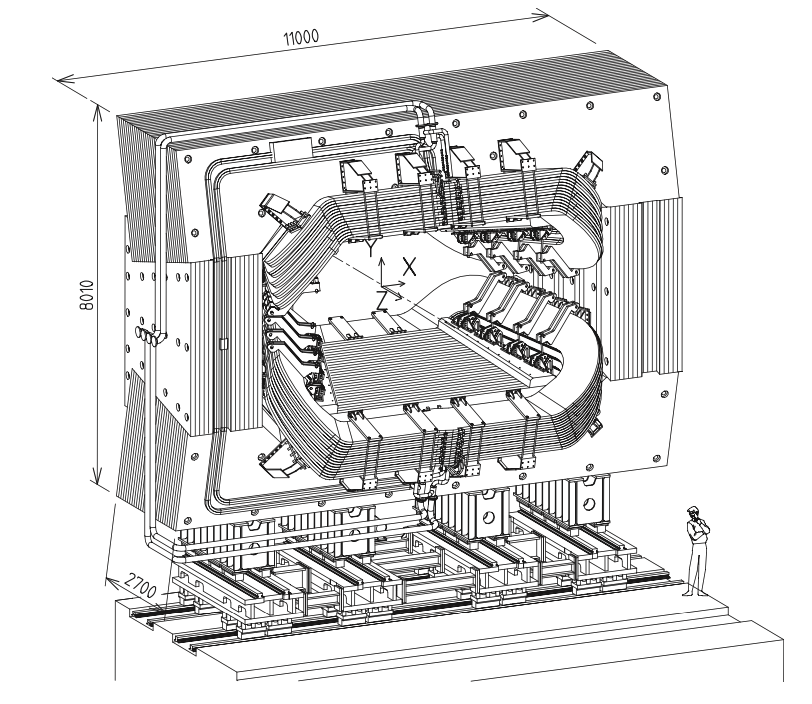
\includegraphics[width=0.75\textwidth]{Figures/02_Detector/MAG}%
	\caption{ Perspective overview of dipole magnet(units in \mm)\supercite{LHCb-DP-2008-001}}
\label{fig:MAG}
\end{figure}



\subsubsection{Silicon Tracker}

Silicon tracker are used in Tracker Turicensis (TT) and the Inner Tracker (IT),
which are constructed by silicon microstrip sensors with a strip pitch of about $200\mum$.
The \ttracker is a planar tracking station, 
which is located upstream of the \lhcb dipole magnet and covers the full acceptance of the experiment, 
as shown in the top of Figure.~\ref{fig:UT}.
The \intr refers to the center region of the three tracking stations downstream of the magnet,
which is 120 \cm wide and 40 \cm, 
as shown in the bottom of Figure.~\ref{fig:UT}.

\begin{figure}[!hbtp]
\centering
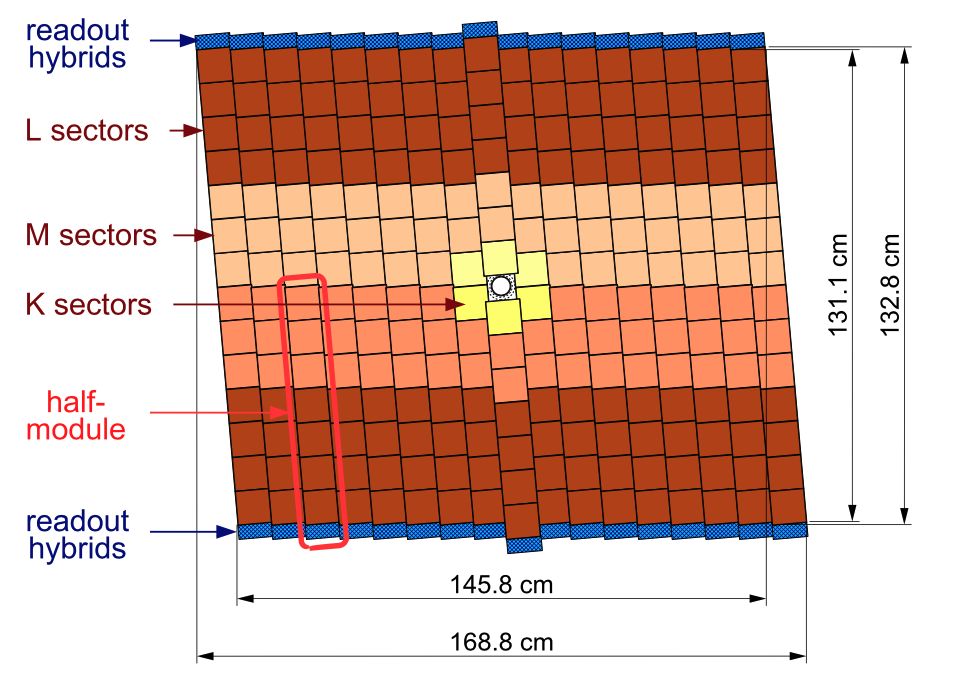
\includegraphics[width=0.7\textwidth]{Figures/02_Detector/UT} \\%
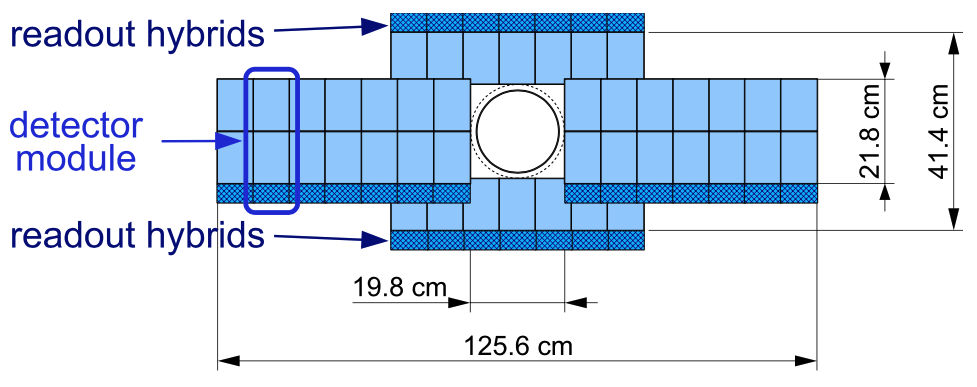
\includegraphics[width=0.65\textwidth]{Figures/02_Detector/IT}%
	\caption{ Overview of the TT (top) and IT (bottom)\supercite{LHCb-DP-2008-001}}
\label{fig:UT}
\end{figure}

The basic building blocks of the TT layers are half modules, 
which cover half of the acceptance and are joined together end-to-end in order to create the full module. 
The half modules are made up of seven silicon sensors, 
which are organized into either two or three readout sectors, 
depending on the proximity to the beampipe. 
The read-out sectors have one, two, three, or four sensors bonded together, 
such that the sectors closer to the beampipe, 
which encounter the higher particle flux, 
have the lower number of sensors bonded together. 
The space above and below the beampipe are each covered by a half module, 
and the regions to the sides are covered by rows of seven full modules in the first two layers and eight full modules in the last two layers. 
To avoid acceptance gaps, adjacent modules are staggered by about 1 \cm in z to allow overlap by a few millimeters in x. 
For the u and v layers, individual modules are rotated by the respective stereo angle. 

The three \intr stations consist of four detector boxes arranged around the beampipe.
A detector box contains four detection layers which are arranged in the same ($x-u-v-x$) configuration as the \ttracker. 
Each of the detection layers has seven silicon modules. 
Acceptance gaps are avoided by having adjacent modules staggered by 4 \mm in the z direction and an overlap by 3 \mm in the x direction. 
The modules in the top and bottom boxes consist of a single silicon sensor, 
while the modules in the side boxes consist of two silicon sensors.


\subsubsection{Outer Tracker}

To keep the costs low, 
the \intr is enclosed by the Outer Tracker (\ot), 
which is a large area straw-tube detector, 
and detects about $70\%$ of the charged particles tracks that are produced inside the LHCb acceptance. 
It has a lower granularity than the ST due to the lower activity in the outer regions. 
Same as the ST it consists of four layers in an (x−u−v−x) arrangement. 
The OT provides excellent momentum resolution which is necessary for the precise determination of the invariant mass of the reconstructed b-hadrons. 
The front-end electronics measure drift times of ionisation clusters produced by charged particles traversing the straw tubes, 
which is translated into hit position. 
Figure.~\ref{fig:TT} shows the three \ot stations which comprise two layers of circular straws with an inner diameter of 4.9 \mm. 
The straws are filled with a mixture of Argon ($70\%$), CO2 ($28.5\%$) and O2 ($1.5\%$) 
to ensure a fast drift time below 50 ns and a sufficient drift-coordinate resolution (200 \mum).

\begin{figure}[!hbtp]
\centering
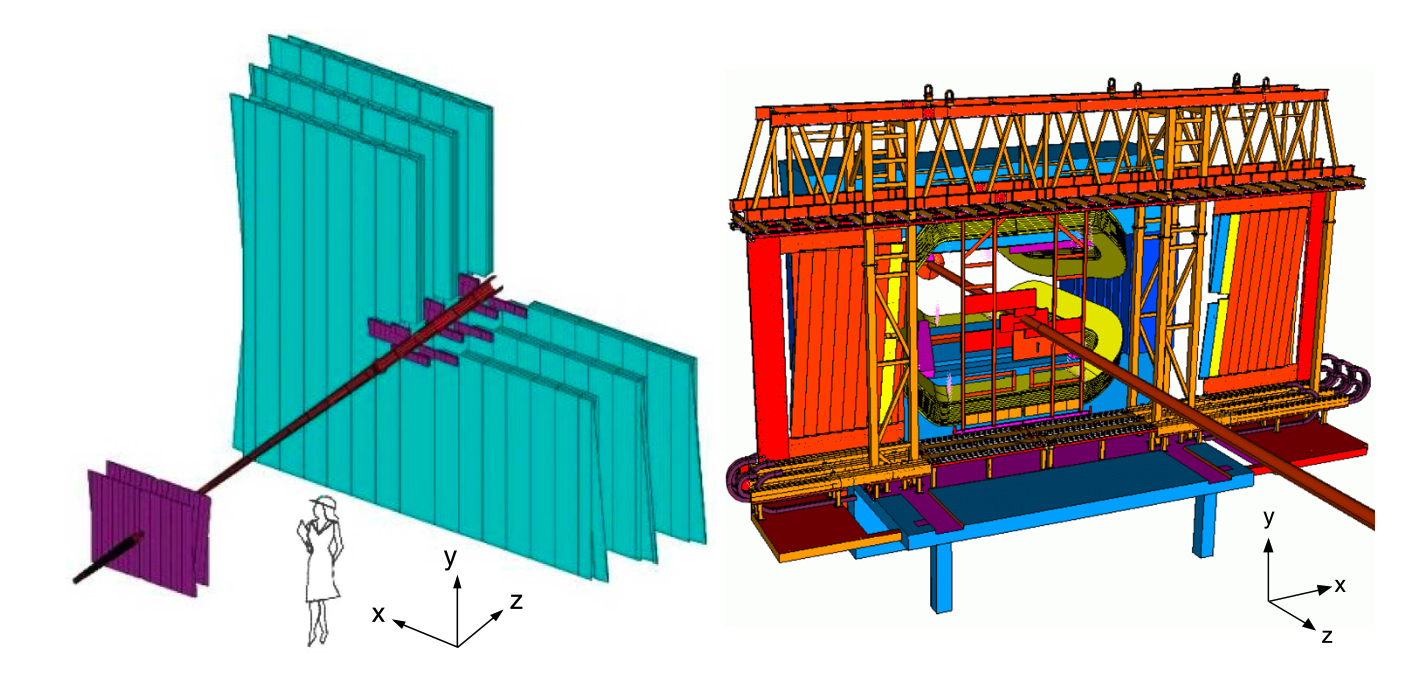
\includegraphics[width=0.99\textwidth]{Figures/02_Detector/TT}%
   \caption{ Left: The three \ot stations surrounding the three \intr stations (purgple). 
	Right: Overview of the \ot bridge carrying the C-frames\supercite{LHCb-DP-2008-001}}
\label{fig:TT}
\end{figure}


All tracking detectors are being upgraded for Run 3. 
The upstream tracker (UT) will use silicon strip technology with improved segmentation and acceptance,
and the total structure is similar to the current one.
The sensors have finer granularity comparing to TT to cope with an increased particle density. 
Sensor strips are vertical to have precise measurement in the horizontal direction,
the direction that charged tracks bend in the dipole magnet.
Each plane is constructed from 16 columnar structure called "staves",
which most have 14 sensor modules,
and mounted alternatively on the front and the back surfaces of its support structure\supercite{LHCb-TDR-015,Proceedings:2015ihx,Rudolph:2020zeq}.

The tracking stations downstream of the magnet will be replaced with a scintillating fiber (SciFi) system during \upgradeone,
which is a total different detector comparing to OT.
The SciFi tracker consists of three stations each with four detection planes. 
The detector is built from individual modules ($0.5\m\times4.8\m$), 
each comprising 8 fibre mats with a length of 2.4\m as active detector material. 
The fibre mats consist of 6 layers of densely packed blue-emitting scintillating fibres with a diameter of 250\mum. 
The scintillation light is recorded with arrays of state-of-the-art multi-channel silicon photomultipliers (SiPMs). 
A custom ASIC is used to digitize the SiPM signals. 
Subsequent digital electronics performs clustering and data-compression before the data is sent via optical links to the DAQ system. 
To reduce the thermal noise of the SiPM, 
in particular after being exposed to a neutron fluence of up to $1012\neqcmcm$, 
expected for the lifetime of the detector, 
the SiPM arrays are mounted in so called cold-boxes and cooled down by 3D-printed titanium cold-bars to $-40\degc$
\supercite{LHCb-TDR-015,Massafferri:2020dbk}.



\subsection{Particle identification}

The purpose of the particle identification (PID) system is to identify the different particle species that travel through the LHCb detector. 
In \proton\proton collisions at the LHC predominantly pions are produced, 
hence it is crucial to distinguish them from the other particle types. 
Information from the Ring Imaging Cherenkov detectors is used to distinguish the charged final state hadrons - kaons, pions, and protons. 
The calorimeters provide information to identify and measure the energy of photons, electrons and hadrons.
The muon detectors are employed to detect and measure muons.


\subsubsection{\rich}

The Ring Imaging CHerenkov (RICH) detectors at LHCb are based on the principle of Cherenkov radiation. 
Cherenkov radiation occurs when a charged particle travels through a medium faster than the speed of light in that medium. 
Cherenkov photons are emitted in a cone shape with opening angle $\theta_{c}$ with respect to the direction of the particles momentum as
\begin{equation}
	cos(\theta_{c}) = \frac{1}{n\beta}
\label{eq:RICH}
\end{equation}
where $n$ is the refractive index of the medium and $\beta=v\/c$, 
where $v$ is the velocity of the particle and $c$ is the speed of light in a vacuum. 

The \rich detectors constains \richone and \richtwo, 
amimg to identify charged tracks with low momentum and high momentum respectively.
The \richone detector is positioned between the \velo and the \ttracker. 
It covers the full angular momentum and provides PID for particles between $1-60\gevc$.
The photodetector planes are split into two halves, 
one above the beam line and one below the beam line. 
The \richtwo covers the full LHCb angular acceptance.
The \richtwo sub-detector is placed between the third tracking station and the first muon station. 
It successfully distinguishes particles with momenta between 15 and 100 \gevc. 
Since high momentum particles are less bent by the magnet, 
the \richtwo detector covers a smaller angular acceptance of 15 mrad up to 100 (120) mrad in the vertical (horizontal) plane. 
The \richtwo Rdetector plane is also made up of two sections, 
placed at either horizontal side of the beam line.
The layout of the \rich detectors is given in Figure~\ref{fig:RICH}. 
The Cherenkov radiation is emitted and reflected out of the detector acceptance by a spherical mirror and a flat mirror. 
They are focused on detection planes, 
where the Cherenkov photons are detected using Hybrid Photon Detectors (HPDs).
Each half of \richone (\richtwo) is equipped with 98 (144) HPDs. 
The particles velocity is reconstructed by identifying rings of Cherenkov photons. 
In combination with the momentum information from the tracking stations, the mass is determined, and the particle can be identified.

\begin{figure}[!hbtp]
\centering
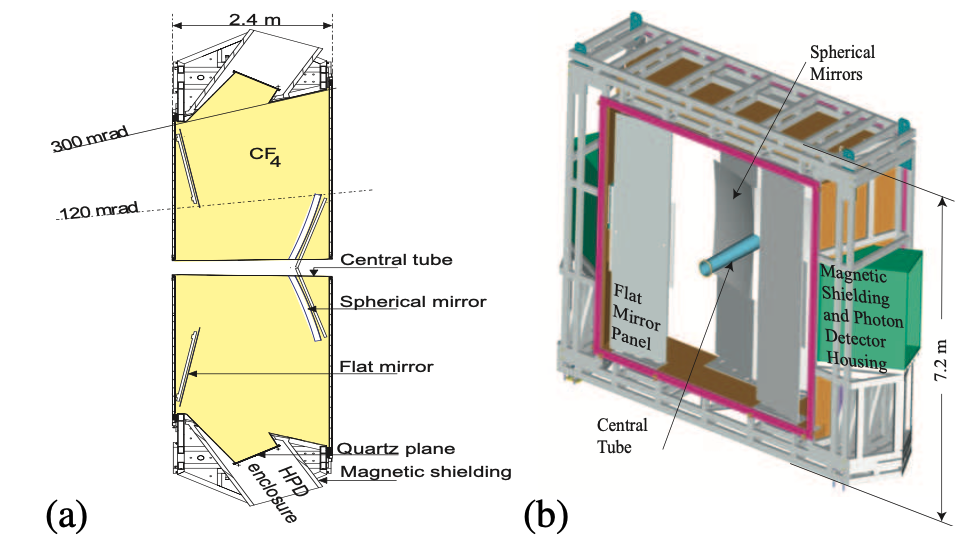
\includegraphics[width=0.85\textwidth]{Figures/02_Detector/RICH}%
   \caption{ Sideview of the \richone detector (Left) and top view of the \richtwo detector\supercite{LHCb-DP-2008-001}}
\label{fig:RICH}
\end{figure}

In order to allow operation of the RICH detector system at the upgrade luminosity,
The \rich detectors is being upgraded by installing new single-photon detectors 
(multianode photomultiplier tubes in place of hybrid photo-detectors) read out by 40 MHz capable electronics, 
and by modifying the upstream RICH optics and mechanics.
The \richone optical system has been redesigned: 
in particular the focal length of the spherical mirrors is increased from 2.7 m to 3.7 m to reduce the hit occupancy on the photodetectors
\supercite{LHCb-TDR-015,FIORINI2020161688}. 
%with the goal of allowing stable operation and easier access to the detector during maintenance.



\subsubsection{Calorimeters}
\label{subsubsec:calorimter}

The main purpose of the calorimeter system is the identification of hadrons, electrons and photons,
and the measurement of their energies and positions.
It is important for calorimeters to enable the reconstruction of $B$-decay channels containing a prompt photon or \piz.
The requirement of a good background rejection and reasonable efficiency for these channels 
adds demanding conditions on the detector performance in terms of resolutions shower separation.

The general structure is that of an electromagnetic calorimeter (\ecal) followed by a hadron calorimeter (\hcal)
as shown in Figure.~\ref{fig:LHCb}.
Besides, 
The scintillator pad detector (\spd) and preshower detector (\presh) are set in the front of \ecal,
the \spd is used to reduce the background for electron trigger,
while the \presh performs to reject the high background of charged particles in \lone trigger.
The \ecal has three zones with different cell size, 
as shown in the left plot of Figure.~\ref{fig:CALO}.
In the inner section, 
the cell size is designed to be close to the Moliere radius, 
which leads most of the energy of a shower deposited in one cell.
The right plot of Figure.~\ref{fig:CALO} shows the lateral segmentation of \hcal, 
which is divided into two zone according to the cell size.
Some propertities to the calorimeter sub-detector are summarized in Table.~\ref{tab:ecal_requirements}.

\begin{figure}[!hbtp]
\centering
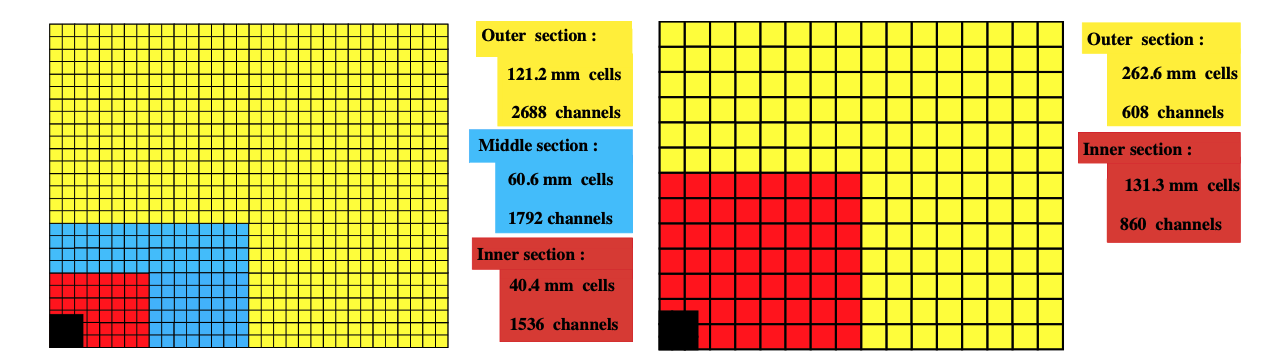
\includegraphics[width=0.99\textwidth]{Figures/02_Detector/CALO}%
   \caption{ The lateral segmentation of the \spd$\slash$\presh and \ecal (left) and the \hcal (right) for a quarter of the detector front\supercite{LHCb-DP-2008-001}}
\label{fig:CALO}
\end{figure}

\begin{table}[h]
\caption{Properties of the calorimeter sub-detector.}
\begin{center}
	\begin{tabular}{c| c|c|c}
\hline \hline
sub-detectors  				&   \spd$\slash$\presh  &  \ecal    		& \hcal  			 	\\
\hline 
number of channels			&   $2\times5952$  	&   $5952$  		&   $1468$    		\\  
overall lateral dimension in x,y	&   $6.2\m\times7.6\m$   &   $6.3\m\times7.8\m$  &   $6.8\m\times8.4\m$ 	         		\\
deppth in z					&   $2\Xrad$   		&   $25\Xrad$  		&   $5.6\NIL$  		     		\\
basic requirements			&   \tabincell{c}{$20-30$ photoelectons\\per \mip}  &  \tabincell{c}{$\sigma(E)/E=$\\$10\%/\sqrt{E}\oplus1.5\%$}   	
	   &   \tabincell{c}{$\sigma(E)/E=$\\$80\%/\sqrt{E}\oplus10\%$}  \\
dynamic range				&   $0-100$ \mip  		&   $0-10$\gev \et  	&   $0-10$\gev\et       	\\
\hline \hline
\end{tabular}
\normalsize
\label{tab:ecal_requirements}
\end{center}
\end{table}

The basic principle for current four detectors is 
that the light generated in scintillator is used to measure the energy deposition, 
which is transmitted by wavelength shifting fibers,
the \ecal will be taken as an example to give more details here.

\begin{figure}[!hbtp]
\centering
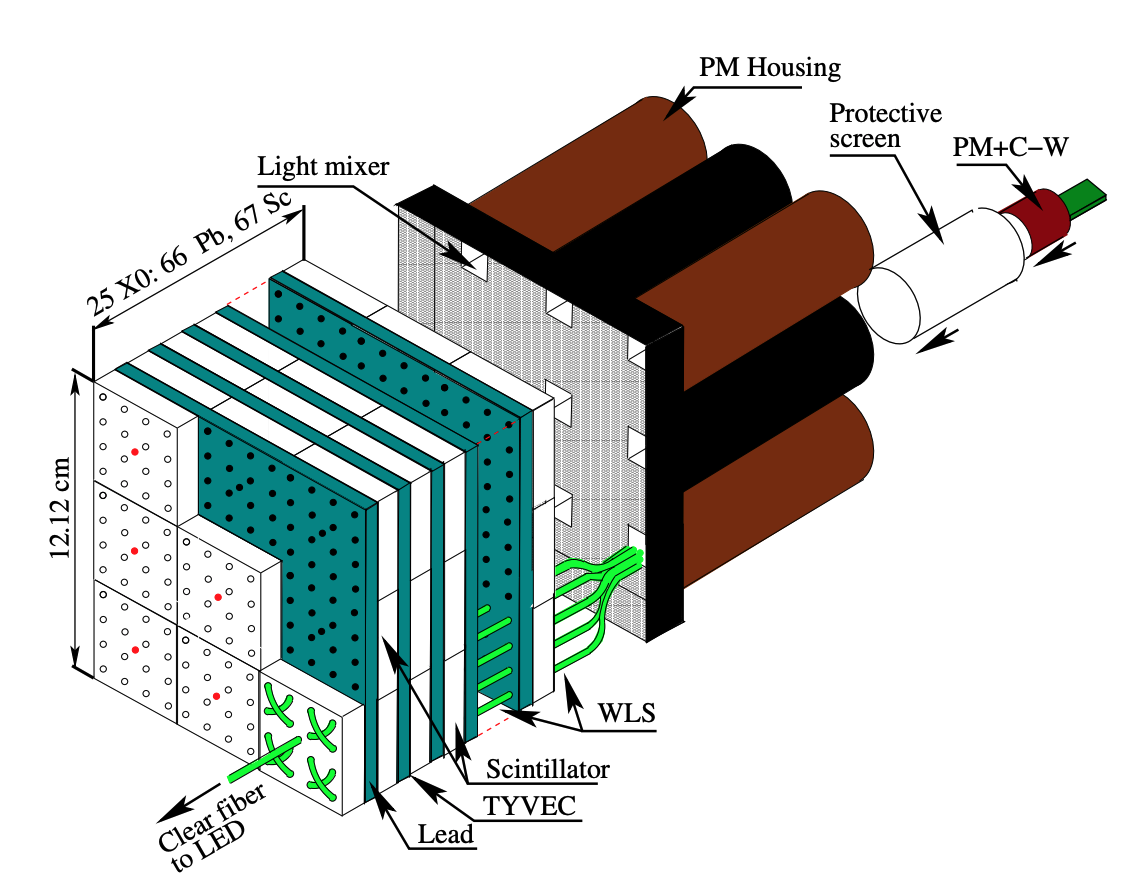
\includegraphics[width=0.49\textwidth]{Figures/02_Detector/Shashlik}%
\caption{ Shashlik construction of \ecal in the inner zone\supercite{Machikhiliyan_2009}}
\label{fig:Shashlik}
\end{figure}

Figure.~\ref{fig:Shashlik} illustrate the construction of \ecal module used in the inner zone.
To set up this sampling calorimeter module, 
total 66 lead plates and 67 scintillator are used,
with the sampling ratio Pb:Sc is $2:4$ (\mm),
stringed by the wavelength-shifting (WLS) fibers.
The WLS is used to transported the light to the photomultipliers (PM),
which can digitize the light signal.
The digitized signal are processed at 40 \mhz rate by the dead-timeless Front-End electronics.
This kind of module is called as shashlik technology.


After the \upgradeone,
the calorimeter system at \lhcb will become very different.
The present \ecal and \hcal will kept,
while the \presh and \spd will be removed as all trigger will perform in software level
\footnote{More details will be discussed in Section.~\ref{sec:trigger}}.
The \ecal and \hcal front-end electronics will be totally rebuilt,
the PM gain will be reduced by factor of 5 to reduce the PM degradation\supercite{LHCb-TDR-014}.

The \hcal will be removed after \upgradetwo,
and the \ecal will be rebuilt using a total new technology.
The specific scheme of \ecal at LHCb is under consideration,
and more details about this will discussed in Chapter.~\ref{chap:ecal}.




\subsubsection{Moun system}

The final part of the LHCb detector is the muon system which provides the identification
of muons. 
The muon system is made of five stations (M1 to M5) covering an angular acceptance of ±300 mrad in the horizontal plane and ±200 mrad in the vertical plane,
as shown in Figure.~\ref{fig:MUON}.
This corresponds to a geometrical efficiency of approximately $46\%$ for the detection
of muons arising from B hadrons. 
The first muon station, M1, 
is placed before the calorimeters in order to avoid possible multiple scattering effects that could modify the
particle trajectory. 
The remaining stations, M2 to M5, 
are placed after the calorimeter system, 
at the end of the LHCb detector, 
and are separated by iron planes 80 cm thick.
Each muon station is divided into four regions (R1-R4) as shown in Fig. 2.19. 
The R1
region is the closest to the beam-pipe and has the most dense segmentation while the R4 region is the farther. 
The segmentation defined per region is such that the charged particle occupancy is expected to be approximately the same in each region. 
All the muon chambers are composed by Multi-Wire Proportional Chambers, 
except for the inner region of the M1 station, 
which exploits three gas electron multiplier foils sandwiched between anode and cathode planes (GEM detectors). 
In total, the muon system consist of 1368 MWPC and 12 GEM detectors.

\begin{figure}[!hbtp]
\centering
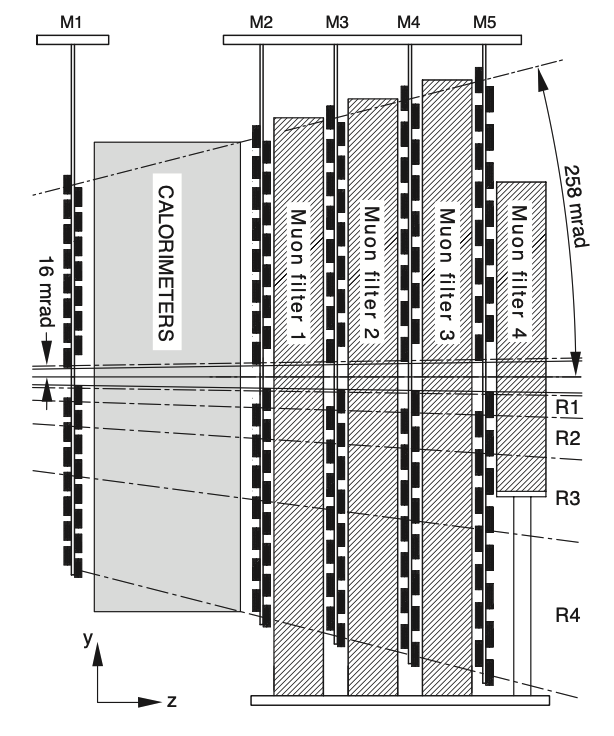
\includegraphics[width=0.65\textwidth]{Figures/02_Detector/MUON}%
\caption{ Sideview of the muon system\supercite{LHCb-DP-2008-001}}
\label{fig:MUON}
\end{figure}

During \upgradeone,
the muon off-detector readout electronics will be redesigned to allow complete event readout at 40 \mhz.
Besides, the M1 before the calorimeter system will be removed\supercite{LHCb-TDR-015,Cardini_2014}.


